\documentclass{article}
\usepackage{physics}
\usepackage{graphicx}
\usepackage{caption}
\usepackage{amsmath}
\usepackage{bm}
\usepackage{framed}
\usepackage{authblk}
\usepackage{empheq}
\usepackage{amsfonts}
\usepackage{esint}
\usepackage[makeroom]{cancel}
\usepackage{dsfont}
\usepackage{centernot}
\usepackage{mathtools}
\usepackage{subcaption}
\usepackage{bigints}
\usepackage{amsthm}
\theoremstyle{definition}
\newtheorem{lemma}{Lemma}
\newtheorem{defn}{Definition}[section]
\newtheorem{prop}{Proposition}[section]
\newtheorem{rmk}{Remark}[section]
\newtheorem{thm}{Theorem}[section]
\newtheorem{exmp}{Example}[section]
\newtheorem{prob}{Problem}[section]
\newtheorem{sln}{Solution}[section]
\newtheorem*{prob*}{Problem}
\newtheorem{exer}{Exercise}[section]
\newtheorem*{exer*}{Exercise}
\newtheorem*{sln*}{Solution}
\usepackage{empheq}
\usepackage{tensor}
\usepackage{xcolor}
%\definecolor{colby}{rgb}{0.0, 0.0, 0.5}
\definecolor{MIT}{RGB}{163, 31, 52}
\usepackage[pdftex]{hyperref}
%\hypersetup{colorlinks,urlcolor=colby}
\hypersetup{colorlinks,linkcolor={MIT},citecolor={MIT},urlcolor={MIT}}  
\usepackage[left=1in,right=1in,top=1in,bottom=1in]{geometry}
\usepackage{newpxtext,newpxmath}
\newcommand*\widefbox[1]{\fbox{\hspace{2em}#1\hspace{2em}}}
\newcommand{\p}{\partial}
\newcommand{\R}{\mathbb{R}}
\newcommand{\C}{\mathbb{C}}
\newcommand{\lag}{\mathcal{L}}
\newcommand{\nn}{\nonumber}
\newcommand{\ham}{\mathcal{H}}
\newcommand{\M}{\mathcal{M}}
\newcommand{\I}{\mathcal{I}}
\newcommand{\K}{\mathcal{K}}
\newcommand{\F}{\mathcal{F}}
\newcommand{\w}{\omega}
\newcommand{\lam}{\lambda}
\newcommand{\al}{\alpha}
\newcommand{\be}{\beta}
\newcommand{\x}{\xi}
\newcommand{\G}{\mathcal{G}}
\newcommand{\f}[2]{\frac{#1}{#2}}
\newcommand{\ift}{\infty}
\newcommand{\lp}{\left(}
\newcommand{\rp}{\right)}
\newcommand{\lb}{\left[}
\newcommand{\rb}{\right]}
\newcommand{\lc}{\left\{}
\newcommand{\rc}{\right\}}
\newcommand{\V}{\mathbf{V}}
\newcommand{\U}{\mathcal{U}}
\newcommand{\Id}{\mathcal{I}}
\newcommand{\D}{\mathcal{D}}
\newcommand{\Z}{\mathcal{Z}}

%\setcounter{chapter}{-1}

\usepackage{enumitem}
\usepackage{listings}
\captionsetup[lstlisting]{margin=0cm,format=hang,font=small,format=plain,labelfont={bf,up},textfont={it}}
\renewcommand*{\lstlistingname}{Code \textcolor{violet}{\textsl{Mathematica}}}
\definecolor{gris245}{RGB}{245,245,245}
\definecolor{olive}{RGB}{50,140,50}
\definecolor{brun}{RGB}{175,100,80}

% 3j symbol
\newcommand{\tj}[6]{ \begin{pmatrix}
		#1 & #2 & #3 \\
		#4 & #5 & #6 
\end{pmatrix}}

%\hypersetup{colorlinks,urlcolor=colby}
\lstset{
	tabsize=4,
	frame=single,
	language=mathematica,
	basicstyle=\scriptsize\ttfamily,
	keywordstyle=\color{black},
	backgroundcolor=\color{gris245},
	commentstyle=\color{gray},
	showstringspaces=false,
	emph={
		r1,
		r2,
		epsilon,epsilon_,
		Newton,Newton_
	},emphstyle={\color{olive}},
	emph={[2]
		L,
		CouleurCourbe,
		PotentielEffectif,
		IdCourbe,
		Courbe
	},emphstyle={[2]\color{blue}},
	emph={[3]r,r_,n,n_},emphstyle={[3]\color{magenta}}
}

\begin{document}

\begin{center}
	\Large{A quick guide to microwave shielding of polar molecules}
\end{center}	

\begin{center}
	\today
\end{center}

\begin{center}
Huan Q. Bui
\end{center}

\section{Background and outline}

Dipolar molecule such as $^{23}$Na$^{40}$K has a body-frame dipole moment of 2.7 Debye. We make the distinction between "body-frame" and "lab-frame" because the even though the molecule is \textit{polar} in the molecule frame, the expectation value of its dipole moment in the lab frame is zero due to rotational symmetry. In order to break this symmetry, we can apply an external electric field, which polarizes the molecule. The expectation value of this induced dipole moment ranges from zero to its maximum of 2.7 Debye depending on the magnitude the external field. This is all one-body physics, which we will understand all of this quantitatively in the next section.

\section{Spherical harmonics and the dipole operator}

\subsection{Spherical decomposition of vectors}
Since molecules have rotational symmetry, it is convenient to go from Cartesian basis to \textit{spherical basis}. Given a unit vector $\hat{\bm{r}}$, we can decompose it into the spherical basis via the relation
\begin{equation}\label{eq:spherical-decomposition}
\sum_m C_{1m}^* \hat{\bm{e}}_m = \sum_m C_{1m} \hat{\bm{e}}_m  = \hat{\bm{r}},
\end{equation}
where
\begin{equation}
 C_{lm}(\theta,\phi) = \sqrt{\f{4 \pi }{2l + 1}} Y_{lm}(\theta,\phi)
\end{equation}
are the $(l,m)$-Racah-normalized spherical harmonics, and 
\begin{equation}
\hat{\bm{e}}_\pm = \mp \f{\hat{\bm{e}}_x \pm i \hat{\bm{e}}_y}{\sqrt{2}};
\quad\quad\quad 
\hat{\bm{e}}_0 = \hat{\bm{e}}_z.
\end{equation}
Proving \eqref{eq:spherical-decomposition} is straightforward: we just need to look up the expressions for $Y_{1m}(\theta, \phi)$ and plug them in explicitly. The left-most term of equation \eqref{eq:spherical-decomposition} is equal to $\hat{\bm{r}}$. Once done, the other equality follows immediately from the fact that $\hat{\bm{r}}$ is real (and therefore the second term is equal to the (conjugate of) the first term). 
\begin{eqnarray}
&&C_{1-}^* \hat{\bm{e}}_{-} + 
C_{10}^* \hat{\bm{e}}_{0}  + 
C_{1+}^* \hat{\bm{e}}_{+} \nonumber \\
&=\,\, &\f{1}{2}e^{+i\phi} \sqrt{\f{3}{2\pi}} \sqrt{\f{4\pi}{3}} \sin\theta  \f{\hat{\bm{e}}_x - i \hat{\bm{e}}_y}{\sqrt{2}} 
	+ \f{1}{2}\sqrt{\f{3}{\pi}} \sqrt{\f{4\pi}{3}} \cos\theta  \hat{\bm{e}}_z 
	+ \f{1}{2}e^{-i\phi} \sqrt{\f{3}{2\pi}} \sqrt{\f{4\pi}{3}} \sin\theta  \f{\hat{\bm{e}}_x + i \hat{\bm{e}}_y}{\sqrt{2}} 
	\nonumber \\
&=\,\, & \sin\theta\cos\phi\, {\hat{\bm{e}}}_x + \sin\theta\sin\phi\, {\hat{\bm{e}}}_y + \cos\theta \,{\hat{\bm{e}}}_z
\nonumber \\
&=\,\, & \hat{\bm{r}}. \quad\quad\quad \checkmark
\end{eqnarray}

\noindent With this formalism, we can now express the dipole interaction $-\hat{\bm{d}} \cdot \bm{E}$ in terms of spherical harmonics. The electric field can be written as 
	\begin{align}
	\bm{E} 
	= E_z \hat{\bm{e}}_z + E_x \hat{\bm{e}}_x + E_y \hat{\bm{e}}_y 
	= E_0 \hat{\bm{e}}_0 + E_+ \hat{\bm{e}}_+ + E_- \hat{\bm{e}}_- 
	= \sum_m E_m^* \hat{\bm{e}}_m = \sum_m E_m \hat{\bm{e}}_m^* 
 	\end{align}
 	where $E_0, E_\pm$ defined in terms of $E_{x,y,z}$ in a similar way as the $\hat{\bm{e}}_{m}$'s are defined in terms of $\hat{\bm{e}}_{x,y,z}$. With this,  
 \begin{eqnarray}
 -\hat{\bm{d}} \cdot \bm{E} 
 &=& -d \hat{\bm{r}} \cdot \mathbf{E} \nn \\
 &=& -d \sum_{m,n} C_{1m}^* E_n \hat{\bm{e}}_m \cdot  \hat{\bm{e}}_n^* \nn\\ 
 &=& -d \sum_{m,n} C_{1m} E_n^* \hat{\bm{e}}_m^* \cdot  \hat{\bm{e}}_n \nn \\
 &=& -d\sum_m C^*_{1m}E_m  \nn \\
 &=& -d\sum_m C_{1m}E_m^*.
 \end{eqnarray}
	
A by-product of this decomposition is the following result: Suppose we have two unit vectors $\hat{\bm{r}}$ and $\hat{\bm{r}}'$ pointing in the direction of solid angle $(\theta,\phi)$ and $(\theta',\phi')$. Let us call $\Theta$ the angle between the vectors, then
\begin{eqnarray}
	\cos\Theta 
	&=& \hat{\bm{r}} \cdot \hat{\bm{r}}' \nn \\
	&=& \sum_{m,n} C_{1m}(\theta,\phi)C_{1n}^*(\theta',\phi')\, \hat{\bm{e}}_m^* \cdot  \hat{\bm{e}}_{n} \nn\\
	&=& \sum_{m,n} C_{1m}(\theta,\phi)C_{1n}^*(\theta',\phi')\delta_{mn} \nn \\
	&=& \sum_m C_{1m}(\theta,\phi)C_{1m}^*(\theta',\phi') \nn \\
	&=& \cos\theta \cos\theta' + \f{1}{2}e^{-i\phi-i\phi'}\sin\theta\sin\theta'+\f{1}{2}e^{i\phi + i\phi'}\sin\theta\sin\theta' \nn \\
	&=& \cos\theta\cos\theta' + \cos(\phi - \phi')\sin\theta\sin\theta',
\end{eqnarray}
as expected from standard geometry. A generalization of this result (for which $l=1$) is 
\begin{equation}
\textcolor{black}{P_l(\cos\Theta) = \sum_m C_{lm}^*(\theta,\phi) C_{lm}(\theta',\phi') }.
\end{equation}
The proof is done by setting one of the unit vectors to be the $z$-axis, and the angles simplify.

\subsection{Spherical harmonics matrix elements}

We also need to know how to evaluate matrix elements involving spherical harmonics. For example, sometimes we want to evaluate how the dipole interaction term $-\hat{\bm{d}} \cdot \bm{E}$ couples different $\ket{J, m_J}$ states. In such cases, we want to evaluate terms of the form
\begin{equation}\label{eq:SH-element}
\langle j_1 m_{1} | Y_{JM} | j_2 m_{2} \rangle = \int \,d\Omega \, Y^*_{j_1 m{1}} Y_{JM} Y_{j_2 m_{2}},
\end{equation}
for which $J=1$ is relevant for dipole transitions, $J=2$ for quadrupole, etc. To do this, we consider two particles with angular momenta $\bm{j}_1$ and $\bm{j}_2$. The total angular momentum is $\bm{J} = \bm{j}_1 + \bm{j}_2$. We can go between the coupled and uncoupled basis via 
\begin{eqnarray}
| (j_1j_2) JM\rangle &=& \sum_{m_1,m_2} |j_1m_1\rangle | j_2m_2\rangle \langle j_1m_1j_2m_2 | JM\rangle\\
|j_1m_1\rangle | j_2m_2\rangle &=& \sum_{J,M} |(j_1j_2)JM\rangle \langle JM| j_1m_1j_2m_2\rangle.
\end{eqnarray}
The Clebsch-Gordan coefficients imply that the sum over $M$ has only one nonzero term $M=m_1+m_2$, and $|j_1-j_2| < J < j_1+j_2$. We also have that the wavefunction of each particle at polar angle $\Omega_i = (\theta_1,\phi_i)$ is 
\begin{equation}
\langle \Omega_i | j_i m_i \rangle = Y_{j_im_i}(\Omega_i).
\end{equation}
For the state of definite total angular momentum $J$, we have
\begin{equation}
\Phi_{JM}(\Omega_1,\Omega_2) = \langle \Omega_1 ,\Omega_2| (j_1j_2)JM\rangle,
\end{equation}
which requires two sets of polar angles $\Omega_1$ and $\Omega_2$. Now, the problem at hand is a one-particle problem. Thus, we reduce the two-particle problem to one-particle by considering the function 
\begin{equation}
F_{JM}(\Omega) \equiv \langle \Omega,\Omega| (j_1j_2)JM\rangle
\end{equation}
where $\Omega_1 = \Omega_2 = \Omega$. This is a wavefunction of \textit{an} effective particle with angular momentum quantum numbers $J,M$. Indeed, it inherits its eigenvalues $\bm{J}^2$ and $J_z$ from $\Phi_{JM}(\Omega_1,\Omega_2)$. Therefore, $F_{JM}(\Omega)$ must be proportional to the spherical harmonic $Y_{JM}(\Omega)$. Let us call
\begin{equation}
F_{JM}(\Omega) = A_{(j_1j_2)J} Y_{JM}(\Omega). 
\end{equation}
The factor $A_{(j_1j_2)J}$ cannot depend on $M$ as $F_{JM}$ must behave exactly like $Y_{JM}$, in particular when acted upon by $J_{\pm}$, which changes $M$. From here we have that
\begin{equation}\label{eq:AY-equation}
A_{(j_1j_2)J} Y_{JM}(\Omega) = \sum_{m_1,m_2}  \langle j_1m_1j_2m_2 | JM\rangle Y_{j_1m_1}(\Omega) Y_{j_2m_2}(\Omega).
\end{equation}

\noindent We can now evaluate the matrix element \eqref{eq:SH-element} in three steps. First, we find $A_{(j_1 j_2) J}$. Next, we find an expression relating 
$Y_{j_1m_1} (\Omega) Y_{j_2 m_2} (\Omega)$ 
to the sum over the $Y_{JM}(\Omega)$. Finally, we put everything together to evaluate \eqref{eq:SH-element}.  \\

\noindent To find $A_{(j_1j_2)J}$ we consider the special case where $\Omega = (\theta=0,\phi)$, where
\begin{equation}
Y_{j_im_i}(\Omega) = Y_{j_im_i}(\theta=0,\phi) = \sqrt{\f{2j_i+1}{4\pi}} \delta_{m_i0}.
\end{equation}
From equation \eqref{eq:AY-equation} we find that
\begin{equation}
A_{(j_1j_2)J} \sqrt{\f{2J+1}{4\pi}} \delta_{M0} = \sum_{m_1,m_2}  \langle j_1m_1j_2m_2 | JM\rangle \sqrt{\f{2j_1+1}{4\pi}} \delta_{m_10} \sqrt{\f{2j_2+1}{4\pi}} \delta_{m_20}.
\end{equation}
This equation is nontrivial if $M=m_1=m_2 = 0$, in which case we can solve for $A_{(j_1j_2)J}$:
\begin{equation}
A_{(j_1,j_2)J} =   \sqrt{\f{(2j_1+1)(2j_2+1)}{4\pi(2J+1)}} \langle j_1 0 j_2 0 | J 0  \rangle.
\end{equation}

\noindent By applying $\langle \Omega,\Omega|$ to the LHS of 
\begin{equation}
|j_1m_1\rangle | j_2m_2\rangle = \sum_{J,M} |(j_1j_2)JM\rangle \langle JM| j_1m_1j_2m_2\rangle,
\end{equation}
we find that
\begin{eqnarray}
{Y_{j_1m_1} (\Omega) Y_{j_2m_2} (\Omega) }
&=& \sum_{J,M} F_{JM}(\Omega) \langle JM| j_1m_1j_2m_2\rangle \nn \\
&=& \sum_{J,M} A_{(j_1j_2)J} Y_{JM}(\Omega) \langle JM| j_1m_1j_2m_2\rangle \nn \\
&=& {\sum_{J,M} \sqrt{\f{(2j_1+1)(2j_2+1)}{4\pi(2J+1)}} \langle j_1 0 j_2 0 | J 0  \rangle  \langle JM| j_1m_1j_2m_2\rangle Y_{JM}(\Omega)}.
\end{eqnarray}

\noindent It remains to evaluate \eqref{eq:SH-element} by plugging things in and using orthonormality of spherical harmonics:
\begin{eqnarray}
{\langle j_3 m_3| Y_{j_2m_2} |j_1m_1\rangle }
&=& \int \,d\Omega \, Y^*_{j_3m_3}(\Omega) Y_{j_2m_2}(\Omega) Y_{j_1m_1}(\Omega) \nn \\
&=& \int \,d\Omega \, Y^*_{j_3m_3}(\Omega) \textcolor{black}{\sum_{J,M} \sqrt{\f{(2j_1+1)(2j_2+1)}{4\pi(2J+1)}} \langle j_1 0 j_2 0 | J 0  \rangle  \langle J M | j_1 m_1 j_2m_2\rangle Y_{JM}(\Omega)} \nn\\
&=& \sqrt{\f{(2j_1+1)(2j_2+1)}{4\pi(2j_3+1)}} \langle j_1 0 j_2 0 | j_3 0  \rangle  \langle j_3 m_3| j_1 m_1 j_2m_2\rangle.
\end{eqnarray}

\noindent This is an example of the Wigner-Eckart theorem. We can also read off selection rules from this result:
\begin{enumerate}
\item We have $m_3 = m_1 + m_2$, which we can interpret this as conservation of $z$-angular momentum. 
\item We must be able to form a triangle of lengths $j_1$, $j_2$, and $j_3$, so $j_3$ must lie between $| j_2 - j_1 | $ and $j_1 + j_2$.
\item In addition, the prefactor $\langle j_1 0 j_2 0 |  j_3 0 \rangle$ implies an additional rule: $j_1 + j_2 - j_3$ must be even. This is the \textit{parity rule}: For the integral over the unit sphere to be non-zero, the product of the three spherical harmonics must be an even function under parity.
\end{enumerate}



\section{Diatomic molecule in a static electric field}

We can think of a diatomic molecule as a symmetric top which has a Hamiltonian $\mathcal{H} = B\mathbf{J}^2$, where $B = B_\text{rot}$ is the rotational constant. The dipole moment operator is $\hat{\mathbf{d}} = d \hat{\mathbf{r}}$ where $d$ is the value of the maximal induced dipole moment (or \textit{permanent dipole moment}). The eigenstates of this system are spherical harmonics. Now, we turn on a static electric field polarized along the $z$-axis, $\bm{E} = E\hat{\bm{e}}_z$. The Hamiltonian then becomes
\begin{equation}
\ham = B \bm{J}^2 - \hat{\bm{d}} \cdot \bm{E}.
\end{equation}
In the $\{ \ket{J m_J} \}$ basis, the matrix elements of this Hamiltonian are:
\begin{eqnarray}
\langle J' m_{J'} | \ham | J m_J \rangle 
&=&  B J(J+1)\delta_{JJ'}\delta_{m_{J'}m_J} - dE \langle J' m_{J'} | C_{10} | J m_J \rangle \nn \\
&=& B J(J+1)\delta_{JJ'}\delta_{m_{J'}m_J} - dE \sqrt{\f{4\pi}{3}} \underbrace{\int \,d\Omega \, Y_{J' m_{J'}}^* Y_{10} Y_{J m_J}} \nn \\
&=& B J(J+1)\delta_{JJ'}\delta_{m_{J'}m_J} -dE  \sqrt{\f{(2J+1)(2+1)}{3(2J'+1)}} \langle (J, 0) (1,0) | (J', 0)  \rangle  \langle J' m_{J'}|(J m_J)(1,0)\rangle \nn \\
&=& B J(J+1)\delta_{JJ'}\delta_{m_{J'}m_J} -dE  \sqrt{\f{(2J+1)(2+1)}{3(2J'+1)}} \langle (J, 0) (1,0) | (J', 0)  \rangle  \langle J' m_{J'}|(J m_J)(1,0)\rangle,
\end{eqnarray}
where we have used the fact that $C_{10} = C_{10}^*$ and remove the conjugation symbol. To get the matrix elements in the second term, we must use Wigner's 3-j symbols:
\begin{equation}
\langle j_1 m_1 j_2 m_2 | J M \rangle = (-1)^{-j_1 +j_2 -M} \sqrt{2J+1} 
\tj{j_1}{j_2}{J}{m_1}{m_2}{-M}
\end{equation}
which with we write the Hamiltonian matrix elements as 
\begin{align}
\langle J' m_{J'} | \ham | J m_J \rangle 
=&\,\,B J(J+1)\delta_{JJ'}\delta_{m_{J'}m_J} \nn \\
&-dE \sqrt{\f{(2J+1)(2+1)}{3(2J'+1)}} 
(-1)^{-J + 1} (-1)^{-J + 1 -m_{J'}} \sqrt{2J'+1} \sqrt{2J'+1} \tj{J}{1}{J'}{0}{0}{0} 
\tj{J}{1}{J'}{m_J}{0}{-m_{J'}} \nn \\
= &\,\, B J(J+1)\delta_{JJ'}\delta_{m_{J'}m_J}  -dE (-1)^{-m_{J'}} \sqrt{\f{(2J+1)(2+1)(2J'+1)}{3}} \tj{J}{1}{J'}{0}{0}{0} \tj{J}{1}{J'}{m_J}{0}{-m_{J'}}.
\end{align}

We can generate this matrix up to some $J_\text{max}$ and diagonalize to find the eigenstates and their energies. We then focus on the lowest-energy state for each value of $dE/B$, which is a mix of the $J=0$ and $(J=1, m=0)$ states. Figure \ref{fig:energies} shows the first six energy levels up to an electric field $E \approx 10B/d$. For this calculation, I have picked $J_\text{max} = 10$.

\begin{figure}[!htb]
		\centering
		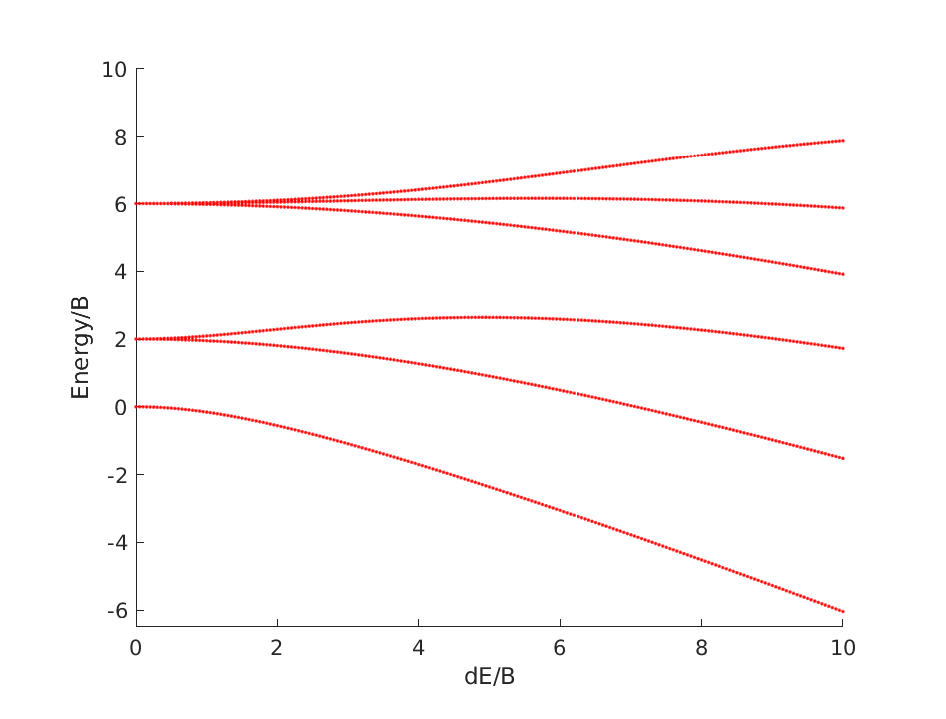
\includegraphics[width=0.7\textwidth]{energies.eps}
		\caption{Energies of the first six energy levels up to an electric field $E \approx 10 B/d$.}
		\label{fig:energies}
\end{figure}

\begin{figure}[!htb]
		\centering
		\begin{subfigure}{.5\textwidth}
			\centering
			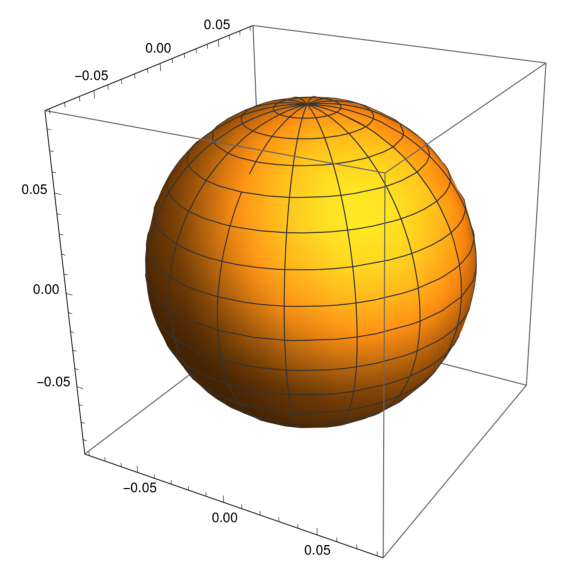
\includegraphics[width=0.9\linewidth]{e0.eps}
			\caption{$\abs{\bra{\theta,\phi}\ket{\Psi}}^2$ for $dE/B=0$.}
			\label{fig:0}
		\end{subfigure}%
		\begin{subfigure}{.5\textwidth}
			\centering
			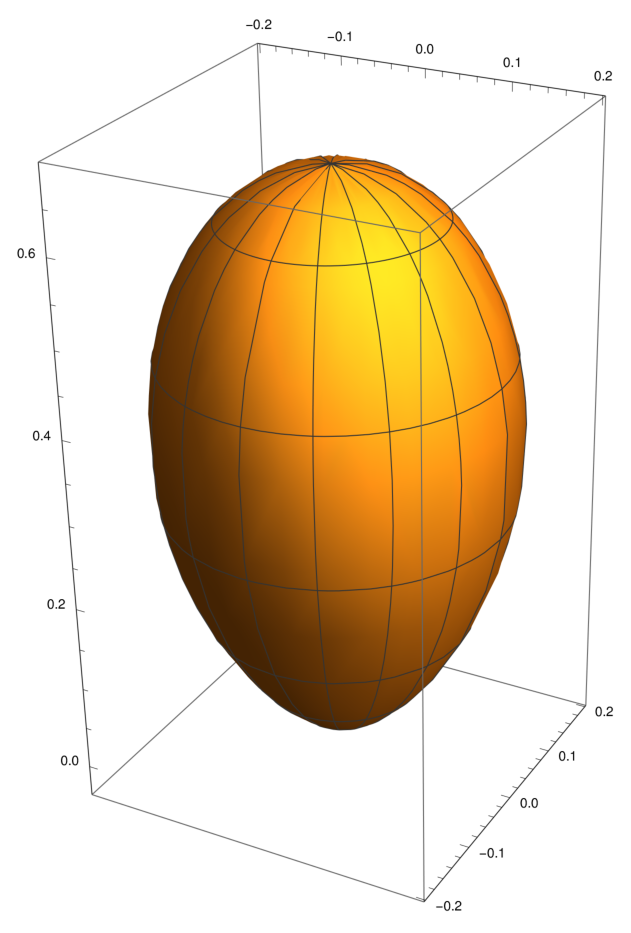
\includegraphics[width=0.75\textwidth]{e10.eps}
			\caption{$\abs{\bra{\theta,\phi}\ket{\Psi}}^2$ for $dE/B=10$.}
			\label{fig:10}
		\end{subfigure}
\end{figure}

MATLAB code for calculating:
	\begin{lstlisting}
	J = 10;
	strength = 0:0.05:10;
	size = (J+1)^2;
	H = zeros(size,size);
	
	% create a basis for the Hamiltonian
	basis = [];
	for j = 0:1:J
	for mj = -j:1:j
	basis = [basis; [j mj]];
	end
	end
	
	%%% first plot energies as a fn of dE/B
	stark = figure(1);
	for a = strength % loop over field strengths
	for r = 1:size
	j = basis(r,1);
	mj = basis(r,2);
	for c = 1:size     
	jj = basis(c,1);  
	mjj = basis(c,2);
	
	H(r,c) = j*(j+1)*(j==jj)*(mj==mjj)...
	-a*(-1)^(-mjj)*sqrt((2*j+1)*(2*1+1)*(2*jj+1)/3)...
	*Wigner3j([j,1,jj],[0,0,0])*Wigner3j([j,1,jj],[mj,0,-mjj]);             
	end
	end
	energies = eig(H);
	hold on 
	plot(a*ones(size), energies, '.', 'Color', 'red', 'MarkerSize',4);
	end
		
	% plot includes up to 6 lowest energies only
	hold off
	ylim([-6.5 10])
	xlabel('dE/B')
	ylabel('Energy/B')
		
	strength = [0 1 10];
	wavefunction = 0;
	
	for a = strength 
	for r = 1:size
	j = basis(r,1);
	mj = basis(r,2);
	for c = 1:size     
	jj = basis(c,1);  
	mjj = basis(c,2);
	
	H(r,c) = j*(j+1)*(j==jj)*(mj==mjj)...
	-a*(-1)^(-mjj)*sqrt((2*j+1)*(2*1+1)*(2*jj+1)/3)...
	*Wigner3j([j,1,jj],[0,0,0])*Wigner3j([j,1,jj],[mj,0,-mjj]);             
	end
	end
	% diag n plot eigenvalues associated with field strength a = dE/B
	[state,energy] = eigs(H,1,'SA');
	disp('Ground state energy:')
	disp(energy)
	disp('Ground state:')
	disp(state) 
	end
\end{lstlisting}


\noindent Mathematica code for plotting:
\begin{lstlisting}
	(*dE/B=0 ---> |0,0> state*)
	
	Energy1 = 0;
	State1 = SphericalHarmonicY[0, 0, \[Theta], \[Phi]];
	SphericalPlot3D[
	Conjugate[State1]*State1, {\[Theta], 0, Pi}, {\[Phi], 0, 2 Pi}, 
	PlotRange -> All]
		
	(*dE/B=10 ---> get superposition state*)
	
	Jmax3 = 4;
	Base3 = Flatten[
	Table[SphericalHarmonicY[J, mJ, \[Theta], \[Phi]], {J, 0, 
	Jmax2}, {mJ, -J, J}], 1];
	
	Energy3 = -6.0448;
	
	State3 = {-0.6477, 0.0000, -0.6782, -0.0000, 
	0.0000, -0.0000, -0.3323, -0.0000, 0.0000, -0.0000, 0.0000, 
	0.0000, -0.0987, -0.0000, -0.0000, 0.0000, 0.0000, 0.0000, -0.0000,
	0.0000, -0.0191, -0.0000, 0.0000, -0.0000, 0.0000};
	
	State3 = State3/Norm[State3];
	
	wfn3 = Dot[Base3, State3]
	
	-0.182713 - 0.33137 Cos[\[Theta]] - 
	0.104805 (-1 + 3 Cos[\[Theta]]^2) - 
	0.0368325 (-3 Cos[\[Theta]] + 5 Cos[\[Theta]]^3) - 
	0.0020205 (3 - 30 Cos[\[Theta]]^2 + 35 Cos[\[Theta]]^4)
	
	SphericalPlot3D[
	Conjugate[wfn3]*wfn3, {\[Theta], 0, Pi}, {\[Phi], 0, 2 Pi}, 
	PlotRange -> All, AspectRatio -> Full]
\end{lstlisting}



\section{Diatomic molecule in a microwave field}

Consider a symmetric top molecule in a truncated Hilbert space of rotational states $| J m_J \rangle \in \{  \ket{00}, \ket{1-1}, \ket{10}, \ket{11}  \}$. Let a $\sigma^+$ microwave field couple the state $\ket{00}$ and $\ket{11}$. The composite Hilbert space is now made up of states $| J m_J N\rangle$, where $N$ is the photon number relative to a large reference photon number $N_0$. The Hamiltonian is 
\begin{align}
\ham
&= \ham_\text{mol} + \ham_\text{MW} + \ham_\text{mol + MW} \nn \\
&= 
\begin{pmatrix}
0 &&&\\
& 2B_\text{rot}&& \\
&& 2B_\text{rot}& \\
&&& 2B_\text{rot} 
\end{pmatrix}
+ 
\begin{pmatrix}
sVd
\end{pmatrix}
+ 
\begin{pmatrix}
fsdv
\end{pmatrix}
\end{align}



\bibliography{microwave-shielding} 
\bibliographystyle{unsrt}	

\end{document}